\chapter{Conditions and Decisions} \label{chp:Conditions}
\epigraph{In any moment of decision, the best thing you can do is the right thing, the next best thing is the wrong thing, and the worst thing you can do is nothing.}{Theodore Roosevelt}

The last chapter introduced some very limited form of interactivity by introducing the possibility to enter values at runtime. We now want to extend this interactivity by breaking out of the \emph{linear flux of control}: up to now, code is executed in exactly the order the code is written, and each line of code is executed. In this chapter, we will introduce ways to break out of this restriction and learn how to tie the execution of parts of our code to \emph{conditions}.

\section{Truth Values} \label{sec:truthvalues}
To arrive at our goal of conditionally executing portions of code, we first need to learn how to formulate a condition. For this, we introduce the mathematical concept of a \emph{truth value}. A mathematical expression can either be \emph{true} or \emph{false}. For example, the expression $1 + 5 \times 8 + 1 = 42$ holds \emph{true}, while $-1 > 1$ is \emph{false}. We can use the computer to evaluate the truthfulness of any expression. For that, we introduce a new set of comparison operators:

{
	\newcolumntype{C}{>{         \centering\arraybackslash} p{.20\linewidth}}
	\newcolumntype{O}{>{\ttfamily\centering\arraybackslash} p{.25\linewidth}}
	\rowcolors{1}{white}{tabhighlight}
\begin{tabularx}
	{\linewidth}
	{CO|CO}
\toprule[1.5pt]

	\textbf{Comparison}     & \normalfont \textbf{Operator Symbol}  &
	\textbf{Comparison}     & \normalfont \textbf{Operator Symbol}
\tabcrlf

	Equality       & ==   &  Inequality         & != \\
	Less than      & <    &  Greater than       & >  \\
	Less or equal  & <=   &  Greater or equal   & >= \\

\bottomrule[1.5pt]
\end{tabularx}
\captionof{table}{Comparison operators in C}\label{tab:OperatorsComparison}
}

Note that for equality, we use a \emph{double equals sign} to distinguish this comparison operation from the value assignment.

This notion of \emph{true} or \emph{false} can be represented with a single bit. But as you know from the last chapter, a processor can ever only handle byte sized chunks of bits. So, in this context, the wasteful approach was used: \emph{false} is represented by the value \inC{0} while any \emph{nonzero} value will be seen as \emph{true}.

With these new operators, we can translate our mathematical expressions into code. They evaluate to an \inC{int}, with which we can perform any operation that we already know. For example, the expression
\begin{center}
\inC{1 + 5 * 8 + 1 == 42}
\end{center}
is a somewhat convoluted way of computing the value \inC{1}.

Since comparisons are simply \inC{int} expressions, we can do computations with them, just like with \enquote{regular maths} expressions, including storing these results in \inC{int} variables:
\begin{codebox}[truthValues.c]
\begin{minted}[linenos]{c}
#include <stdio.h>

int main () {
    int x     = 17;
    int truth = (x > 5) + (x < 5) + (x == 17);

    printf("%d true expressions.\n", truth);
}
\end{minted}
\captionof{code}{Storing turth values}
\end{codebox}

\begin{cmdbox}[Output: truthValues.c]
\begin{minted}{text}
2 true expressions.
\end{minted}
\end{cmdbox}

In this example, the three parentheses are evaluated one after another, yielding \inC{1} for \texttt{x > 5}, \inC{0} for \texttt{x < 5} and \inC{1} for \texttt{x == 17}. The three subexpressions are then summed up to give the result \inC{2}.

This is actually a thing we rarely ever do; but understanding helps us develloping a deep understanding how decision making works in a computer.

\begin{warnbox}[Symbols \texttt{true} and \texttt{false}]
In principle, you are free to use variables named \texttt{true} or \emph{false}. However, I strongly recommend against it. There are plenty of libraries (extensions to the C language) that define these symbols to mean \inC{1} or \inC{0}, respectively. They do so because expressions like \texttt{motorIsTurnedOn() == true} are just easier on human eyes than \texttt{motorIsTurnedOn() == 1}.

Defining the symbols to be constants with exactly these values is so common that when programmers see a piece of code with either of these symbols in it, they don't look up the definition, but simply assume that the symbols \emph{abide by the convention}. Going against this convention is a great way of confusing and annoying fellow coders.

While C does allow you to assign any value to the symbols \texttt{true} and \texttt{false}, most other programming languages don't. In C++, C\#, Java, Groovy and Python\footnote{In Python, the symbols actually are \texttt{True} and \texttt{False}, with a captial as a first letter. Still, The two words have a very strict definition in the programming community.}, they are \emph{reserved keywords}, \ie they are hard coded into the language itself. This is just one more reason not to adapt an unhealthy habit.
\end{warnbox}

\section{Conditional Execution of Code: \inC{if}}
\subsection{Simple \inC{if}}
Now that we know how to give answers to yes/no questions, we can tie portions of code to these answers. The keyword \inC{if} introduces an if...then block: \emph{if} some condition holds true, \emph{then} do things. In it's simplest form, this can be achieved with the following syntax:

\begin{codebox}[Syntax: Simple \texttt{if} block]
\begin{minted}{c}
if (condition) {
    statements
}
\end{minted}
\end{codebox}

In this, \texttt{condition} is anything that can be evaluated to a truth value. Usually, it is a comparison like \inC{x > 5}; but since truth values are essentially only numbers, any expression that evaluates to a number may be put here.

\texttt{statements} is one or several lines of code, \eg value assignments (\inC{x = 7 + y;}) or calls to functions (\inC{printf("hello world\n");}. These lines are executed as normal, but \emph{only if} \texttt{condition} \emph{is true}. Otherwise, they are skipped over, and the lines after the \inC{if} block are executed, \ie the lines after the closing curly brace \texttt{\}}.

Let's look at an example:
\begin{codebox}[evenNumbers.c]
\begin{minted}[linenos]{c}
#include <stdio.h>

int main () {
    int foobar = 0;

    printf("Please enter an integer: ");
    scanf("%d", &foobar);

    if (foobar % 2 == 0) {
        printf("%d is an even number.\n", foobar);
    }

    printf("You entered %d.\n", foobar);
}
\end{minted}
\captionof{code}{Detecting and handling even numbers}
\end{codebox}

\begin{tcbraster}[raster columns=2,
                  raster equal height,
                  nobeforeafter,
                  raster column skip=0.2cm]
\begin{cmdbox}[Possible Output: evenNumbers.c]
\begin{minted}{text}
Please enter an integer: 5
You entered 5.
\end{minted}
\end{cmdbox}
%
\begin{cmdbox}[Possible Output: evenNumbers.c]
\begin{minted}{text}
Please enter an integer: 4
4 is an even number.
You entered 4.
\end{minted}
\end{cmdbox}
\end{tcbraster}

First we remember that the modulus operator \texttt{\%} computes the remainder of a division. If divided by 2, even numbers will have a remainder of zero, otherwise they will have a remainder of 1. So, in line 9 we really do ask whether the value of \texttt{foobar} is even. If and only if this is the case, we execute line 10. Otherwise, we jump ahead to the end of the \inC{if} block. The block began with the opening curly brace \texttt{\{} in line 9, and ends with its closing counterpart \texttt{\}} in line 11. The code outside of the \inC{if} block is always executed, regardless of the truth value.

\begin{warnbox}[Pet Peeve: \texttt{if} \enquote{loops}]
When discussing programming with beginners, I often hear the expression \inC{if} \emph{loops}. Please internalize that this wording is \emph{simply and completely wrong}. There is no such thing as \inC{if} \emph{loops}.

A loop is a structure that we'll discuss in detail in chapter \ref{chp:loops} and that allows to jump back in the code and execute the same code several times over. So, the \enquote{trajectory} through the code looks like a loop. Loops share a syntactical similarity with \inC{if} \emph{blocks} in that the looped part is enclosed in braces and initiated by a statement that comprises of a condition; this superficial similarity, however, is the only thing linking \inC{if} \emph{blocks} to loops.

So please, for the love of ones and zeros, do not even start using this abomination of an expression, and rather refer to the structure we're discussing in this chapter as an \inC{if} \emph{block}, or simply an \inC{if} statement.
\end{warnbox}



\begin{warnbox}[Common mistake: Comparison operator \texttt{==} vs. assignment operator \texttt{=}]
It is not uncommon to put an assignment (\texttt{=}) in lieu of a comparision in the condition of an \inC{if} block. \emph{Syntactically}, this makes sense: an assignment does have a return value that usually also is a valid truth value. \emph{Semantically}, it is in by far the most cases wrong -- assigning a value within an \inC{if} condition is hardly ever what we want. At best, it is a sign of bad style. At worst, it is plain wrong and produces a hard to find bug. For that reason, let's see how this bug looks like and how to spot it:
%\end{warnbox}
%%
%\begin{warnbox}[]

\begin{warnbox}[accidentalAssignment.c, leftupper=7mm]
\begin{minted}[linenos]{c}
#include <stdio.h>

int main () {
   unsigned int rowCount = 0;
   printf("Number of rows:\n");
   scanf("%u", &rowCount);

   if (rowCount = 0) {
      printf("Error: cannot create empty table\n");
   }

   printf("Length of table: %d\n", rowCount);
}
\end{minted}
\captionof{code}{accidental assignment in an \texttt{if} block}
\end{warnbox}

This produces the following behaviour:

\begin{cmdbox}[Possible output: accidentalAssignment.c]
\begin{minted}{text}
Number of rows:
5
Length of table: 0
\end{minted}
\end{cmdbox}

As mentioned before, line 8 does not compare \texttt{rowCount} to \inC{0} but assigns the value to the variable. The \emph{return value} of this assignment is the assigned value -- \ie the value \inC{0}, which in the context of the \inC{if} block becomes the truth value \emph{false}. Consequently, we do not see the message \texttt{Error: cannot create empty table}, but find an inconsistent state in line 12.

If you use the compiler flag \texttt{-Wall}, you will see a warning on compilation:

\begin{cmdbox}[Compilerwarnung: accidentalAssignment.c]
\begin{minted}{text}
accidentalAssignment.c: In function ‘main’:
accidentalAssignment.c:9:8: warning: suggest parentheses around assignment 
    used as truth value [-Wparentheses]
    if (rowCount = 0) {
        ^~~~~~~~
\end{minted}
\end{cmdbox}
\end{warnbox}

\begin{hintbox}[Style: Indention and position of braces]
I hope you noticed that I indented the code in the \inC{if} blocks, \ie I put additional four white spaces before the instruction in the \inC{if} block. We are currently only looking at very short codes of negligible complexity, so we could do without these indentations. We will, however, soon get to a level where this extra visual clue to the \emph{structure of our code} becomes an indespensable tool for our devellopment activities. So I want to double down on the fact \emph{that} you should make indentations whenever you open a block statement -- like \inC{if} -- and remove the indentation at the end of a block.

As to \emph{how} you make these indentations, there is no fixed rule that all programmers agree to and abide by. The number of whitespaces per indentation level varies from one through eight, and some prefer tabs instead of whitespaces. Likewise, some coders prefer putting the opening brace in the same line as the statement that \enquote{causes} the block (as I do), while others rather put the opening brace in a line of its own right. There are merits to both options. Some programmers like to advertise their style with almost religious zeal, and discussions can become very emotional, as shown in figure \ref{fig:IndentStyle}.

Whatever your preference in style may be, I will ask you to abide by these rules at the very least:
\begin{itemize}
\item Do make indentations to provide visual clues for the structure of your code
\item Keep your code uniform in look by maintaining the same kind of indentation per level and same position of braces (end of line or own line) for an entire project
\item Never change the indentation style of your colleagues
\end{itemize}
\end{hintbox}

\begin{figure}
	\href{http://www.sandraandwoo.com/2015/04/13/0674-there-are-10-types-of-programmers/}{
		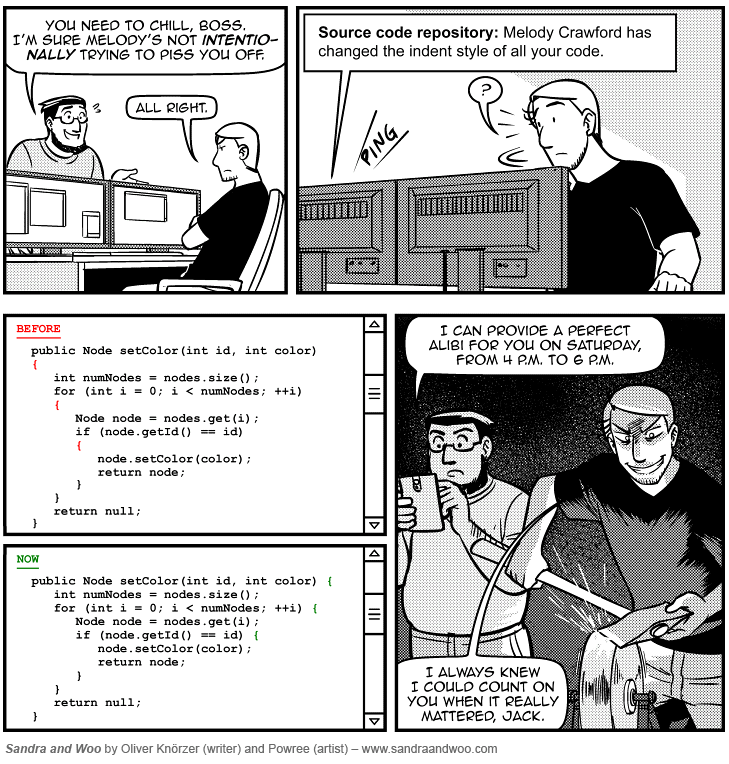
\includegraphics[width=\linewidth]{./gfx/SW-indent-style}
	}
	\caption{A realistic scenario} \label{fig:IndentStyle}
\end{figure}

If there is only a single line of code that should be tied to the condition, then the \texttt{\{}curly braces\texttt{\}} can be ommitted. The above example can thus also be shortened to:
\begin{codebox}[evenNumbers.c]
\begin{minted}[linenos]{c}
#include <stdio.h>

int main () {
    int foobar = 0;

    printf("Please enter an integer: ");
    scanf("%d", &foobar);

    if (foobar % 2 == 0)
        printf("%d is an even number.\n", foobar);

    printf("You entered %d.\n", foobar);
}
\end{minted}
\captionof{code}{Detecting and handling even numbers}
\end{codebox}

You may think of not having to type braces for one line \inC{if} blocks as a useful addition to the language. However, I strongly advise you against omitting braces, even in case of one line blocks. The reason for this advice is that it is not uncommon to amend code after it's written. If you do add lines of code to an \inC{if} block, you will have to remember adding the braces as well -- which you are very likely to forget. Even worse, the indentation that is supposed to help us to grasp the outline of our project will even conceal the error by guiding the eye and suggesting that the code has braces where there are none.

Regard this code listing \ref{code:missingBraces}:
\begin{warnbox}[missingBraces.c, leftupper=7mm]
\begin{minted}[linenos]{c}
#include <stdio.h>

int main () {
    int foo = 0;

    printf("Please enter an integer:\n");
    scanf("%d", &foo);

    if (foo % 2 == 0)
        printf("%d is an even number.\n", foo);
        printf("%d is divisible by 2.\n", foo);

    printf("You entered %d.\n", foo);
}
\end{minted}
\captionof{code}{Incorrect \texttt{if} block (missing braces)} \label{code:missingBraces}
\end{warnbox}

As intended, line 10 is only executed if \texttt{foo} is even; line 11 on the other hand will \emph{always} be executed (like lin 13), regardless of the parity of \texttt{foo}. The indentation however, suggests that it, too, is tied to the condition in line 9.

If you add the braces as soon as you type \inC{if} you cant forget it when you later edit and amend the compound statement:
\begin{codebox}[correctedBraces.c]
\begin{minted}[linenos,firstnumber=9]{c}
    if (foo % 2 == 0) {
        printf("%d is an even number.\n", foo);
        printf("%d is divisible by 2.\n", foo);
    }
\end{minted}
\captionof{code}{Corrected \texttt{if} block (added braces)}
\end{codebox}



\subsection{\inC{if}-\inC{else}}
We can expand the syntax of \inC{if} blocks by an \inC{else} clause. As you'd expect, the statements in this block are executed only if the condition in the \inC{if} condition is \emph{not} satisfied.

\begin{codebox}[Syntax: \texttt{if}-\texttt{else} block]
\begin{minted}{c}
if (condition) {
    statements_true
} else {
    statements_false
}
\end{minted}
\end{codebox}

In a full code example, this could look like so:
\begin{codebox}[ifElse.c]
\begin{minted}[linenos]{c}
#include <stdio.h>

int main () {
    int foo = 0;
  
    printf("Please enter an integer:\n");
    scanf("%d", &foo);

    if (foo % 2 == 0) {
        printf("%d is an even number.\n", foo);
    } else {
        printf("%d is an odd number.\n", foo);
    }
}
\end{minted}
\captionof{code}{\texttt{if}-{else} Blocks}
\end{codebox}

\begin{hintbox}[Bare numbers as conditions (1)]
We've learned that truth values are actually only numbers in special disguise. So whenever we test whether some expression evaluates to zero, we can omit the comparison operator, thereby creating marginally faster code, since the computer has to do one less computation step (computing the truth value). In that sense, we can re-write the former example:

\begin{codebox}[ifElseImplicitComparison.c]
\begin{minted}[linenos, firstnumber=7]{c}
    // ...
    
    if (foo % 2) {
        printf("%d is an odd number.\n", foo);
    } else {
        printf("%d is an even number.\n", foo);
    }
}
\end{minted}
\captionof{code}{\texttt{if}-{else} without explicit comparison}
\end{codebox}

We removed the \texttt{== 0} from line 9. Note that this also required flipping the true- and false case: \texttt{foo \% 2} is true when \texttt{foo} is odd, while \texttt{foo \% 2 == 0} was true when \texttt{foo} is even.
\end{hintbox}

You can nest \inC{if} blocks to almost arbitrary depth
\footnote{According to the C standard, \ie the rules according to which a C compiler has to be programmed, at least 127 levels of nested \texttt{if}s must be supported by the compiler (cf. \url{https://www.open-std.org/JTC1/SC22/WG14/www/docs/n2310.pdf}. The gcc seems to only give an error message if you nest 6200 levels (cf. \url{https://stackoverflow.com/questions/764307/what-limits-the-number-of-nested-loops-in-c}), which should be way beyond any limit of practicality.}.
Hence, we can also implement sub-conditions, that are only evaluated if a primary condition was satisfied. In the following example, we test the parity of numbers again, but limit ourselves to positive numbers:

\begin{codebox}[ifElseNested.c]
\begin{minted}[linenos]{c}
#include <stdio.h>

int main () {
    int foo = 0;
  
    printf("Please enter a positive integer:\n");
    scanf("%d", &foo);

    if (foo > 0) {
        if (foo % 2 == 0) {
            printf("%d is an even number.\n", foo);
        } else {
            printf("%d is an odd number.\n", foo);
        }
    } else {
        printf("%d is an invalid number.\n", foo);
    }
}
\end{minted}
\captionof{code}{Nested \texttt{if}-{else}}
\end{codebox}

Compare this to a -- syntactically valid -- version of the code without any indentations, and you will see why I put so much stress on the value of clear indentation:

\begin{warnbox}[ifElseNestedNotIndented.c, leftupper=7mm]
\begin{minted}[linenos]{c}
#include <stdio.h>
int main () {
int foo = 0;  
printf("Please enter a positive integer:\n");
scanf("%d", &foo);
if (foo > 0) {
if (foo % 2 == 0) {
printf("%d is an even number.\n", foo);
} else {
printf("%d is an odd number.\n", foo);
}} else {
printf("%d is an invalid number.\n", foo);
}}
\end{minted}
\captionof{code}{Nested \texttt{if}-{else} without indentations}
\end{warnbox}


\subsection{More than two cases in one \inC{if} block}
Sometimes we need to identify one of more than cases and act accordingly. If so, nested \inC{if}s are a viable means. In such a scenario, we can combine \inC{else} with a subsequent \inC{if} into a new structure\footnote{Technically, this is an application of the rule that one-line statements need no braces around them: \inC{if (condition_2) {statements}} is a one-line statement, even if \texttt{statements} takes up multiple lines. The braces bundle them together in one compound statement. Technically... \url{https://xkcd.com/1475/}}.:

\begin{codebox}[Syntax: Multi-case \texttt{if}-\texttt{else} block]
\begin{minted}{c}
if (condition_1) {
    statements_1
} else if (condition_2) {
    statements_2
} else if /* ... arbitrarily many else if blocks ... */ {
    statements_n
} else {
    statements_else
}
\end{minted}
\end{codebox}

In this form, we first evaluate \texttt{condition\_1}. If it is satisfied, the computer executes \texttt{statements\_1} and then jumps right to the end of the entire structure, \ie after the \texttt{else}, even if there are other conditions that would be met.

We can illustrate how this works in an example:

\begin{codebox}[ifMultiCase.c]
\begin{minted}[linenos]{c}
#include <stdio.h>

int main () {
    int playerCount = -1;
    printf("How many players are there?\n");
    scanf("%d", &playerCount);

    if      (playerCount < 3) {printf("That's too few players.\n")}
    else if (playerCount > 8) {printf("That's too many players.\n")}
    else                      {printf("Great! Here are the rules: ...\n");}
}
\end{minted}
\captionof{code}{Multiple cases in an \texttt{if} block}
\end{codebox}

Here you see some code that does not perform as naively expected:
\begin{warnbox}[inaccessibleCode.c, leftupper=7mm]
\begin{minted}[linenos]{c}
#include <stdio.h>

int main () {
   int foo = 0;

   printf("Please enter an integer:\n");
   scanf("%d", &foo);

   if        (foo >  5) {
      printf("%d is greater than five.\n", foo);
   } else if (foo > 10) {
      printf("This line will never be printed on screen.\n");
   } else {
      printf("%d is less than five..\n" , foo);
   }
}
\end{minted}
\captionof{code}{inaccessible code in a multi-case \inC{if} structure}
\end{warnbox}

\begin{cmdbox}[Possible Output: inaccessibleCode.c]
\begin{minted}{text}
Please enter an integer
50
50 is greater than five.
\end{minted}
\end{cmdbox}

The condition in line 11 is only ever evaluated, if the one in line 9 was already false. If the first condition \texttt{foo > 5} was true, then after printing \texttt{\%d is greater than five.}, code execution jumps right down to line 16, \ie the end of the code in this example.

\begin{defbox}[Flux of Control]
Lines 9-15 of the above code can be visualized in this flowchart:
\begin{center}
\begin{tikzpicture}
	[
		startstop/.style={rectangle, rounded corners, minimum width=3cm, minimum height=1cm,text centered, draw=black, fill=green!30!blue!30},
		decision/.style={diamond, minimum width=3cm, minimum height=1cm, text centered, draw=black, fill=violet!30},
		process/.style={rectangle, minimum width=4.5cm, minimum height=1cm, text centered, draw=black, fill=yellow!30},
		arrow/.style={thick,->,>=stealth}
	]
	
	\node (enter) at (0, 9) [startstop] {line 7 (\emph{before} \texttt{if})};
	
	\node (cond1) at (0, 6) [decision]  {\texttt{foo > 5}?};
	\node (cond2) at (0, 3) [decision]  {\texttt{foo > 10}?};
	
	\node (if_1) [process] at (5, 6) {line 10 (\enquote{greater than five})};
	\node (if_2) [process] at (5, 3) {line 12 (\enquote{greater than ten})};
	\node (else) [process] at (5, 0) {line 14 (\enquote{less than five})};
	
	\node (eif_1) at (8, 6) {};
	\node (eif_2) at (8, 3) {};
	\node (eelse) at (8, 0) {};
	
	\node (leave) at (8, -2) [startstop] {line 16 (\emph{after} \texttt{if})};
	
	\draw [arrow] (enter)  -- (cond1);
		
	\draw [arrow] 
		(cond1) -- 
		node [text width=1.2cm, midway, align=center] 
			{\color{green!70!black} yes \\ \phantom{.}}
		(if_1);
	
	\draw [arrow] 
		(cond1) -- 
		node [text width=1.2cm, midway, align=left] 
			{\color{red!70!black} no}
		(cond2);
		
	\draw [arrow] 
		(cond2) -- 
		node [text width=1.2cm, midway, align=center] 
			{\color{green!70!black} yes \\ \phantom{.}}
		(if_2);
	
	\draw [arrow] 
		(cond2) |- 
		node [text width=1.2cm, midway, align=left] 
			{\color{red!70!black} no}
		(else);
	
	\draw [arrow] (if_1) -| (leave);
	\draw [arrow] (if_2) -- (eif_2);
	\draw [arrow] (else) -- (eelse);
	\draw [arrow] (eif_1) -- (leave);
\end{tikzpicture}
\end{center}
\captionof{figure}{Flux of control in an \texttt{if}..\texttt{else if} block}

\vspace{3pt}
There is no logically possible path leading to \emph{line 12}, because it would have to pass through \texttt{foo > 5} with \emph{no} and through \texttt{foo > 10} with \emph{yes}.
\end{defbox}


\section{Logical Operators} \label{sec:OperatorsLogical}
Sometimes, execution of a piece of code should depend on more than one condition. For example, before writing a file, it has to be made sure that enough storage space is availabe \emph{and} that the filename is valid. We could achive this by nesting \inC{if} statements:

\begin{codebox}[andNested.c]
\begin{minted}[linenos, firstnumber=420]{c}
    // ...
    
    if (availableDiskSpace < 1024) {
        if (countOfInvalidCharactersInFilename > 0) {
            printf("Error: Could not write file!\n");
        }
    }
    
    // ...
\end{minted}
\captionof{code}{Nested \inC{if} to realize a logical and}
\end{codebox}

But I am pretty sure, you already noticed that we could also collapse this into a single \inC{if} statement by using the \emph{and} operation from the previous chapter. A comparison like \texttt{<} or \texttt{>} produces an integer, which is either 1 or zero. We can join several ones and zeros with the bitwise operators \texttt{\&}, \texttt{|} and \texttt{\textasciicircum}. Thus, the same result is achieved by this code:
\begin{codebox}[andBitwise.c]
\begin{minted}[linenos, firstnumber=420]{c}
    // ...
    
    if ((availableDiskSpace < 1024) & (countOfInvalidCharactersInFilename > 0)) {
        printf("Error: Could not write file!\n");
    }
    
    // ...
}
\end{minted}
\captionof{code}{Bitwise operator joins two conditions in an \inC{if} statement} \label{code:bitwiseAndIf}
\end{codebox}

For reasons I will explain in the next few paragraphs, in such a situation we would prefer \emph{logical operators} over \emph{bitwise operators}. Each of the bitwise operators (\emph{and}, \emph{or}, \emph{xor} and \emph{not}) has a logical counterpart. Both kinds of operators perform the same principle operations; \emph{true and true} will always give \emph{true}, no matter whether you perform a bitwise or a logical \emph{and}. The primary difference between the two is that the logical operators first reduce their operands to \emph{booleans}, i.e. to a single true/false value.

The \emph{bitwise} and between \texttt{11 == 1011$_2$} and \texttt{7 == 0111$_2$} is \texttt{3 == 0011$_2$}. The \emph{logical} and, on the other hand, is simply \texttt{1} or \emph{true}, because both operands \texttt{11} and \texttt{7} are nonzero and therefore count as \emph{true}. Table \ref{tab:logicalAndBitwiseOperators} shows which symbols are used for which operation:

{
\newcolumntype{N}{>{         \centering\arraybackslash} p{.15\linewidth}}
\newcolumntype{R}{>{\ttfamily\centering\arraybackslash} p{.25\linewidth}}
\begin{center}
\rowcolors{1}{white}{tabhighlight}
\begin{tabularx}
	{.73\linewidth}
	{NRR}
\toprule[1.5pt]

    \textbf{Operation} & \textrm{\textbf{Bitwise Operator}}  &  \textrm{\textbf{Logical Operator}}
\tabcrlf
    and &               \& & \&\& \\
    or  &               |  & ||   \\
    xor & \textasciicircum & !=   \\
    not & \textasciitilde  & !    \\

\bottomrule[1.5pt]
\end{tabularx}
\end{center}
\captionof{table}{Logical and bitwise operators in C}\label{tab:logicalAndBitwiseOperators}
}

Note that it is not a mistake to put the inequality operator \texttt{!=} in the table as the logical xor operator. If you compare to the behaviour listed in table \ref{tab:booleanLogic}, you will find that \emph{inequality} is exactly what a logical xor tests for.

So, why should we write
\mint{c}{if ((availableDiskSpace < 1024) && (countOfInvalidCharactersInFilename > 0))}
instead of using a bitwise operator like in code listing \ref{code:bitwiseAndIf}?

In day-to-day life, the principal reason is semantics: using a logical operator says that we really only care about yes-or-no information; bitwise operators on the other hand imply that some black magic on individual bits is happening\footnote{which usually makes experienced coders nervous}. They also allow treating values in themselves as truth values. Compare these two pieces of code:
{
\begin{tcbraster}[raster columns=2,
                  raster equal height,
                  nobeforeafter,
                  raster column skip=0.2cm]
\begin{codebox}[nonzeroLogicalAnd.c]
\begin{minted}[linenos, firstnumber=69]{c}
if (x && y) {
  printf("Both x and y are nonzero.");
}
\end{minted}
\end{codebox}
%
\begin{codebox}[nonzeroBitwiseAnd.c]
\begin{minted}[linenos, firstnumber=69]{c}
if ((x != 0) & (y != 0)) {
  printf("Both x and y are nonzero.");
}
\end{minted}
\end{codebox}
\end{tcbraster}
\captionof{code}{Bitwise and logical conjunction for nonzero-test}
}

The left example using the logical and works in this shortened form no matter what values \texttt{x} and \texttt{y} store. For the bitwise operators, on the other hand, an explicit comparison to zero is needed\footnote{You might still find the right hand side form easier to understand due to its explicitness, and this point of view has its merit. Of course, you can always combine both versions, \ie use logical operators with explicit comparisons.} (think of the example \texttt{x = 1} and \texttt{y = 2}. Without the explicit comparison, the bitwise \emph{and} would give \texttt{0} or false).

Another major difference is the fact that the bitwise \emph{and} and \emph{or} are \emph{short circuited}. This means that the computer tries to save some time by evaluating the second operand only when this is necessary. You know that for an \emph{and}, both operands need to be \emph{true}. If the left hand side operand is already known to be \emph{false}, we automatically know that the result of the \emph{and} will always be \emph{false}, no matter what comes to the right of it. This can be used to prevent nonsensical operations:
\begin{codebox}[Example: preventDivByZero.c]
\begin{minted}[linenos, firstnumber=69]{c}
if (x && (y / x > 5)) {
    printf("Treshold surpassed");
}
\end{minted}
\captionof{code}{Short circuiting}
\end{codebox}

We know that a division by zero is ill-defined. This also holds for programming in C: a program trying to divide by zero will usually crash\footnote{unless you are using floating point numbers... but more on that in chapter \ref{chp:misc}.}, which is obviously bad. For that reason, we should always make sure the denominator of a division is nonzero. In the above example, due to the short circuiting behavior of the logical \emph{and}, the expression \texttt{y / x} is only evaluated if \texttt{x} itself was already nonzero.

In a similar manner, the logical or (\texttt{||}) evaluates its right hand side operand only if the left hand side was \emph{false}, because \emph{true or anything} will always be \emph{true}.

\begin{hintbox}[Rule of thumb: two character operators with \texttt{if}]
We already encountered the fact that the assignment operator (\texttt{=}) is usually misplaced in an \inC{if} statement. We have seen that confusing the bitwise operators with the logical ones can have unintended consequences, too.

While it sadly does not always hold, I recommend you to adopt the rule of thumb: \emph{an \inC{if} requires a two-character operator} (\ie \texttt{==}, \texttt{\&\&}, ...). Notable exceptions from this rule are \texttt{<}, \texttt{>} and \texttt{!}, and every time you do evil bit hacking.
\end{hintbox}

\begin{hintbox}[Bare numbers as conditions (2)]
Whether or not a number is nonzero is a question we have to answer very often in programming. We've already learned that we can drop the explicit comparision to zero when the code we want to run code if some number is \emph{nonzero}. With the logical \emph{not}, we can also run code only when it is \emph{zero}:

\vspace{6pt}
\begin{codebox}[implicitIfZero.c]
\begin{minted}[linenos]{c}
#include <stdio.h>

int main () {
    unsigned int rowCount = 0;
    printf("Number of rows:\n");
    scanf("%u", &rowCount);

    if (!rowCount) {
        printf("Error: cannot create empty table\n");
    }
}
\end{minted}
\captionof{code}{logical not to test for zero values}
\end{codebox}
\end{hintbox}

In particular using the \emph{or} conjunction can help reduce redundant code. Regard the following example:
{
\begin{tcbraster}[raster columns=2,
                  raster equal height,
                  nobeforeafter,
                  raster column skip=0.2cm]
\begin{warnbox}[ifSequence.c, leftupper=7mm]
\begin{minted}[linenos]{c}
#include <stdio.h>

int main () {
    unsigned int playerCount = 0;

    printf("number of players:\n");
    scanf("%u", &playerCount);

    if (playerCount < 2) {
        printf(
            "Game not apt for %d ",
            playerCount
        );
        printf("players.\n");
    }

    if (playerCount > 5) {
        printf(
            "Game not apt for %d ",
            playerCount
        );
        printf("players.\n");
    }
}
\end{minted}
\end{warnbox}
%
\begin{codebox}[ifConjunction.c]
\begin{minted}[linenos]{c}
#include <stdio.h>

int main () {
    unsigned int playerCount = 0;

    printf("number of players:\n");
    scanf("%u", &playerCount);

    if ((playerCount < 2) ||
        (playerCount > 5)
       ) {
        printf(
            "Game not apt for %d ",
            playerCount
        );
        printf("players.\n");
    }
}
\end{minted}
\end{codebox}
\end{tcbraster}
\captionof{code}{Avoiding redundant code with logical operators}
}

Not only is the right hand side code much shorter; it is also easier to maintain and debug. If we later want do more than only print a warning that a given player number is not suitable, in the left hand code we need to edit in these changes in two places, and are therefore twice as likely to make typos or (most dangerously) can outright forget to edit the second \inC{if} statement.

\begin{hintbox}[Avoid redundant code]
Whenever you feel like copy-pasting your code, always think twice whether there is not a possibility to restructure your code such that you avoid redundancy. Experience shows that you always spend \emph{way longer} to find and fix bugs due to redundancy than it takes to refactor your code into a more maintainable form.
\end{hintbox}

\section{Many cases: \inC{switch}}


\rule{\textwidth}{2pt}
\newpage
%TODO

%exos:
% - why is 5 & 2 false?
% - which of these are equivalent ~> modus tollens; !!x and (x != 0)

\section{Fallunterscheidungen: \inC{switch}}
Das Schlüsselwort \inC{switch} wird benutzt, um Fallunterscheidungen mit vielen einzelnen Fällen umzusetzen. Die Form von \inC{switch}-Blöcken lautet:

\begin{codebox}[Syntax: \texttt{switch}]
\begin{minted}{c}
switch (Ausdruck) {
   case Wert1 :
      Anweisungen;
      break;
   case Wert2 :
      Anweisungen;
      break;
   ...
   default:
      Anweisungen;
      break;
}
\end{minted}
\end{codebox}

\texttt{Ausdruck} ist dabei ein beliebiger Ausdruck, der zu einer \emph{Ganzzahl} ausgewertet werden kann. Fließkommawerte oder andere Datentypen werden von \inC{switch} leider nicht unterstützt. Dasselbe gilt für \texttt{Wert1}, \texttt{Wert2}, \ldots; jedoch müssen diese Ausdrücke bereits zur \emph{Compile-Zeit} feststehen. Das bedeutet, dass \texttt{Wert1}, \texttt{Wert2}, \ldots keine Variablen oder Elemente enthalten dürfen, die erst bei Ausführung des Programms (zur \emph{Laufzeit}) feststehen.

Wenn die Aussage \texttt{Ausdruck == Wert1} wahr ist, wird der Code unter der entsprechenden \inC{case}-Zeile ausgeführt. Entsprechendes gilt für \texttt{Wert2}, \ldots. Gilt für keinen der angegebenen Werte Gleichheit, so werden die Anweisungen unter \inC{default} ausgeführt.

In der Anwendung kann dies so aussehen:

\begin{codebox}[Beispiel: Menü mit \texttt{switch}]
\begin{minted}[linenos]{c}
#include <stdio.h>

int main () {
   int selection = -1;

   printf("Bitte wählen Sie einen Menüpunkt:\n");
   printf("  1) Spiel starten\n");
   printf("  2) Optionen\n");
   printf("  3) Highscore zeigen\n");
   printf("  0) Beenden\n");

   scanf("%d", &selection);

   switch (selection) {
      case 1 :
         // Code für: Spiel Starten
         break;
      case 2 :
         // Code für: Optionen
         break;
      case 3 :
         // Code für: Highscore
         break;
      case 0 :
         // Code für: Beenden
         break;
      default:
         printf("Ungültige Eingabe!\n");
         break;
   }
}
\end{minted}
\end{codebox}

Der \inC{default}-Teil ist optional. Lässt man diesen weg und trifft keine der \inC{case}-Klauseln zu, so wird nichts ausgeführt -- die Ausführung des Codes wird am Ende des \inC{switch}-Blocks fortgesetzt.

Die Werte zu den \inC{case}-Klauseln dürfen im selben \inC{case}-Block nur jeweils ein einziges Mal vorkommen.

Man kann sich \inC{switch}-Blocks als Kurzform für \inC{if}-Blocks vorstellen\footnote{Die tatsächliche Umsetzung ist etwas komplexer und enthält einige Optimerungsschritte, die hier nicht besprochen werden können. Diese interne Umsetzung ist der Grund, weswegen \inC{switch} nur mit Ganzzahlen funktioniert.}. Das vorige Beispiel lässt sich auch so programmieren:

\begin{codebox}[Beispiel: Menü mit \texttt{if}]
\begin{minted}[linenos]{c}
#include <stdio.h>

int main () {
   int selection = -1;

   printf("Bitte wählen Sie einen Menüpunkt:\n");
   printf("  1) Spiel starten\n");
   printf("  2) Optionen\n");
   printf("  3) Highscore zeigen\n");
   printf("  0) Beenden\n");

   scanf("%d", &selection);

   if        (selection == 1) {
      // Code für: Spiel Starten
   } else if (selection == 2) {
      // Code für: Optionen
   } else if (selection == 3) {
      // Code für: Highscore
   } else if (selection == 0) {
      // Code für: Beenden
   } else {
      printf("Ungültige Eingabe!\n");
   }
}
\end{minted}
\end{codebox}

Wichtig ist das Schlüsselwort \inC{break}. Mit diesem Befehl wird eine Kontrollstruktur wie ein \inC{switch}-Block verlassen und die Codeausführung wird hinter dem aktuellen Block fortgesetzt. Betrachten Sie das folgende Beispiel:

\begin{warnbox}[Beispiel: \texttt{switch} ohne \texttt{break}, leftupper=7mm]
\begin{minted}[linenos]{c}
#include <stdio.h>

int main () {
   int x = 1;

   switch (x) {
      case 0 :
         printf("0\n");
      case 1 :
         printf("1\n");
      case 2 :
         printf("2\n");
      case 3 :
         printf("3\n");
      default :
         printf("d\n");
   }
}
\end{minted}
\end{warnbox}

Das Ergebnis dieses Codes ist:
\begin{cmdbox}[Ausführungsbeispiel: \texttt{switch} ohne \texttt{break}]
\begin{minted}{text}
1
2
3
d
\end{minted}
\end{cmdbox}

Wie zu erwarten springt die Ausführung mit \inC{switch} von Zeile 6 nach Zeile 9. Da hier aber keine \inC{break}s gesetzt wurden, \enquote{fällt die Ausführung durch die \inC{case}-Klauseln}. Das bedeutet, dass am Ende der \inC{case}-Klausel \texttt{1} die Code-Ausführung in Zeile 11 fortgesetzt wird, und somit alle \texttt{printf}-Anweisungen ausgeführt werden. Wird der Compiler mit der Option \texttt{-Wimplicit-fallthrough} gestartet, so finden Sie in der Compiler Ausgabe eine entsprechende Warnung:

\begin{cmdbox}[Compiler-Warnung: \texttt{switch} ohne \texttt{break}]
\begin{minted}{text}
myProgram.c: In function ‘main’:
myProgram.c:8:7: warning: this statement may fall through
[-Wimplicit-fallthrough=]
       printf("0\n");
       ^~~~~~~~~~~~~
myProgram.c:10:5: note: here
     case 1 :
     ^~~~
...
\end{minted}
\end{cmdbox}

Kontrollstrukturen wie \inC{switch} und \inC{if} können (nahezu) beliebig tief ineinander verschachtelt werden.

\section{Kombinierte Fallunterscheidung und Wertzuweisung -- der Ternäre Operator \texttt{?}}
Nicht selten soll der Wert einer Variablen von einer Bedingung abhängen. Wir kennen bisher die Form

\begin{codebox}[Beispiel: Bedingte Wertzuweisung mit \texttt{if}]
\begin{minted}[linenos]{c}
int main () {
   int Bedingung = 1, Variable;

   if (Bedingung) {
      Variable = 1;
   } else {
      Variable = 2;
   }
}
\end{minted}
\end{codebox}

Diese von einer Bedingung abhängige Wertzuweisung kann auch kompakt in einer einzelnen Zeile geschrieben werden. Mit dem \emph{ternären Operator}\footnote{von \emph{ternär}: das Dritte. Dieser Operator braucht drei \emph{Argumente}. Die Addition \texttt{+} ist beispielsweise ein \emph{binärer} Operator, da sie zwei Argumente braucht -- eben die beiden Zahlen, die addiert werden sollen.} \texttt{?} lässt sich dieser Code auch schreiben als:

\begin{codebox}[Beispiel: Bedingte Wertzuweisung mit dem ternären Operator]
\begin{minted}[linenos]{c}
int main () {
   int Bedingung = 1, Variable;

   Variable = Bedingung ? 1 : 2;
}
\end{minted}
\end{codebox}

Wie bereits bei \inC{if} ist \texttt{Bedingung} ein Ausdruck, dem ein Wahrheitswert zugeordnet werden kann. Ist \texttt{Bedingung} erfüllt, so wird der Ausdruck direkt hinter dem \texttt{?} ausgewertet und zugewiesen. Andernfalls wird der Ausdruck hinter dem \texttt{:} verwendet.

Variablen, die in \texttt{Bedingung} vorkommen, können auch in den Rückgabewerten vorkommen. So lässt sich beispielsweise die Betragsfunktion folgendermaßen implementieren:

\begin{codebox}[Beispiel: Betrag einer Zahl  mit dem ternären Operator]
\begin{minted}[linenos]{c}
int main () {
   int x = -42;

   x = x >= 0 ? x : -x;
}
\end{minted}
\end{codebox}
